\chapter{Regression and Reconstruction on Cartesian Product Graphs} 

\label{chap:reg_and_rec} 

\lhead{Chapter 4. \emph{Regression and Reconstruction on Cartesian Product Graphs}} 


 
\section{Graph Products}

\label{sec:reg_and_rec_intro}

In this chapter, we turn our attention to the topic of signal processing on \textit{Cartesian product graphs}. This special class of graph finds applications in numerous areas, such as video, hyper-spectral image processing and network time series problems. However, the Cartesian product is not the only way to consistently define a product between two graphs. In this section we formally introduce the concept of a graph product, examine  some prominent examples, and explain why we choose to look specifically at the Cartesian graph product. 

\subsection{Basic definitions}

In the general case, consider two undirected graphs $\mathcal{G}_A = (\mathcal{V}_A, \mathcal{E}_A)$ and $\mathcal{G}_B = (\mathcal{V}_B, \mathcal{E}_B)$ with vertex sets given by $\mathcal{V}_A = \{a \in \mathbb{N} \, | \, a \leq A \}$ and $\mathcal{V}_B = \{b \in \mathbb{N} \, | \, b \leq B \}$ respectively. (In this context we do not regard zero to be an element of the natural numbers). A new graph $\mathcal{G}$ can be constructed by taking the product between $\mathcal{G}_A$ and $\mathcal{G}_B$. This can be generically written as follows. 

\begin{equation}
    \mathcal{G} = \mathcal{G}_A \, \diamond \, \mathcal{G}_B = (\mathcal{V}, \, \mathcal{E})
\end{equation}

For all definitions of a graph product, the new vertex set $\mathcal{V}$ is given by the Cartesian product of the vertex sets of the factor graphs, that is
 
\begin{equation}
    \mathcal{V} = \mathcal{V}_A \times \mathcal{V}_B = \{(a, \, b) \in \mathbb{N}^2 \, | \, a \leq A \; \text{and} \; b \leq B \}
\end{equation}


Typically, vertices are are arranged in lexicographic order, in the sense that $(a, b) \leq (a', b')$ iff $a < a'$ or ($a = a'$ and $b \leq b'$) \citep{Harzheim2005}. Each consistent rule for constructing the new edge set $\mathcal{E}$ corresponds to a different definition of a graph product. In general, there are eight possible conditions for deciding whether two nodes $(a, b)$ and $(a', b')$ are to be connected in the new graph.

\begin{table}[h]
\def\arraystretch{1.5}
\centering
\begin{tabular}{lclc}
1. & $[a, \, a'] \in \mathcal{E}_A$ & and &  $b = b'$  \\
2. & $[a, \, a'] \notin \mathcal{E}_A$  & and &  $b = b'$  \\
3. & $[a, \, a'] \in \mathcal{E}_A$ & and &  $[b, \, b'] \in \mathcal{E}_B$ \\
4. & $[a, \, a'] \notin \mathcal{E}_A$ & and &  $[b, \, b'] \in \mathcal{E}_B$  \\
5. & $[a, \, a'] \in \mathcal{E}_A$ & and & $[b, \, b'] \notin \mathcal{E}_B$  \\
6. & $[a, \, a'] \notin \mathcal{E}_A$ & and & $[b, \, b'] \notin \mathcal{E}_B$  \\
7. & $a = a'$ & and & $[b, \, b'] \in \mathcal{E}_B$,  \\
8. & $a = a'$ & and &  $[b, \, b'] \notin \mathcal{E}_B$ 
\end{tabular}
\end{table}



Each definition of a graph product corresponds to the union of a specific subset of these conditions, thus, there exist 256 different types of graph product \citep{Barik2015}. Of these, the Cartesian product (conditions 1 or 7), the direct product (condition 3), the strong product (conditions 1, 3 or 7) and the lexicographic product (conditions 1, 3, 5 or 7) are referred to as the standard products and are well-studied \citep{Imrich2000}. A graphical depiction of the standard graph products is shown in figure \ref{fig:graph_products}. In each of these four cases, the adjacency and Laplacian matrices of the product graph can be described in terms of matrices relating to the factor graphs \citep{Fiedler1973, Barik2018}. This is shown in table \ref{tab:grap_product_matrices}. 

\begin{table}[h]
\def\arraystretch{1.8}
\centering
\small
\vspace{0.5cm}
\begin{tabular}{|l|cc|}
    \hline 

    & Adjacency matrix
    & Laplacian \\

    \hline

    Cartesian 
    & $\A_A \oplus \A_B$ 
    & $\LL_A \oplus \LL_B$ \\

    Direct 
    & $\A_A \otimes \A_B$  
    & $\D_A \otimes \LL_B + \LL_A \otimes \D_B - \LL_A \otimes \LL_B$ \\
    
    Strong 
    & $\A_A \otimes \A_B + \A_A \oplus \A_B$ 
    & $\D_A \otimes \LL_B + \LL_A \otimes \D_B - \LL_A \otimes \LL_B + \LL_A \oplus \LL_B$ \\

    Lexicographic 
    & $\I_A \otimes \A_B + \A_A \otimes \J_A$ 
    &  $\I_A \otimes \LL_B + \LL_A \otimes \J_B + \D_A \otimes (B \I_B - \J_B)$ \\

    \hline

\end{tabular}
\vspace{0.2cm}
\caption[The adjacency and Laplacian matrices for the standard graph products]{The adjacency and Laplacian matrices for the standard graph products. Here, $\D_A$ and $\D_B$ are the diagonal degree matrices, i.e $\D_A = \diag{\A_A \mathbf{1}}$. $\I_A$ and $\J_A$ are the $(A \times A)$ identity matrix and matrix of ones respectively. } 
\vspace{0.3cm}
\label{tab:grap_product_matrices}
\end{table}

\begin{figure}[t]
    \begin{center}
    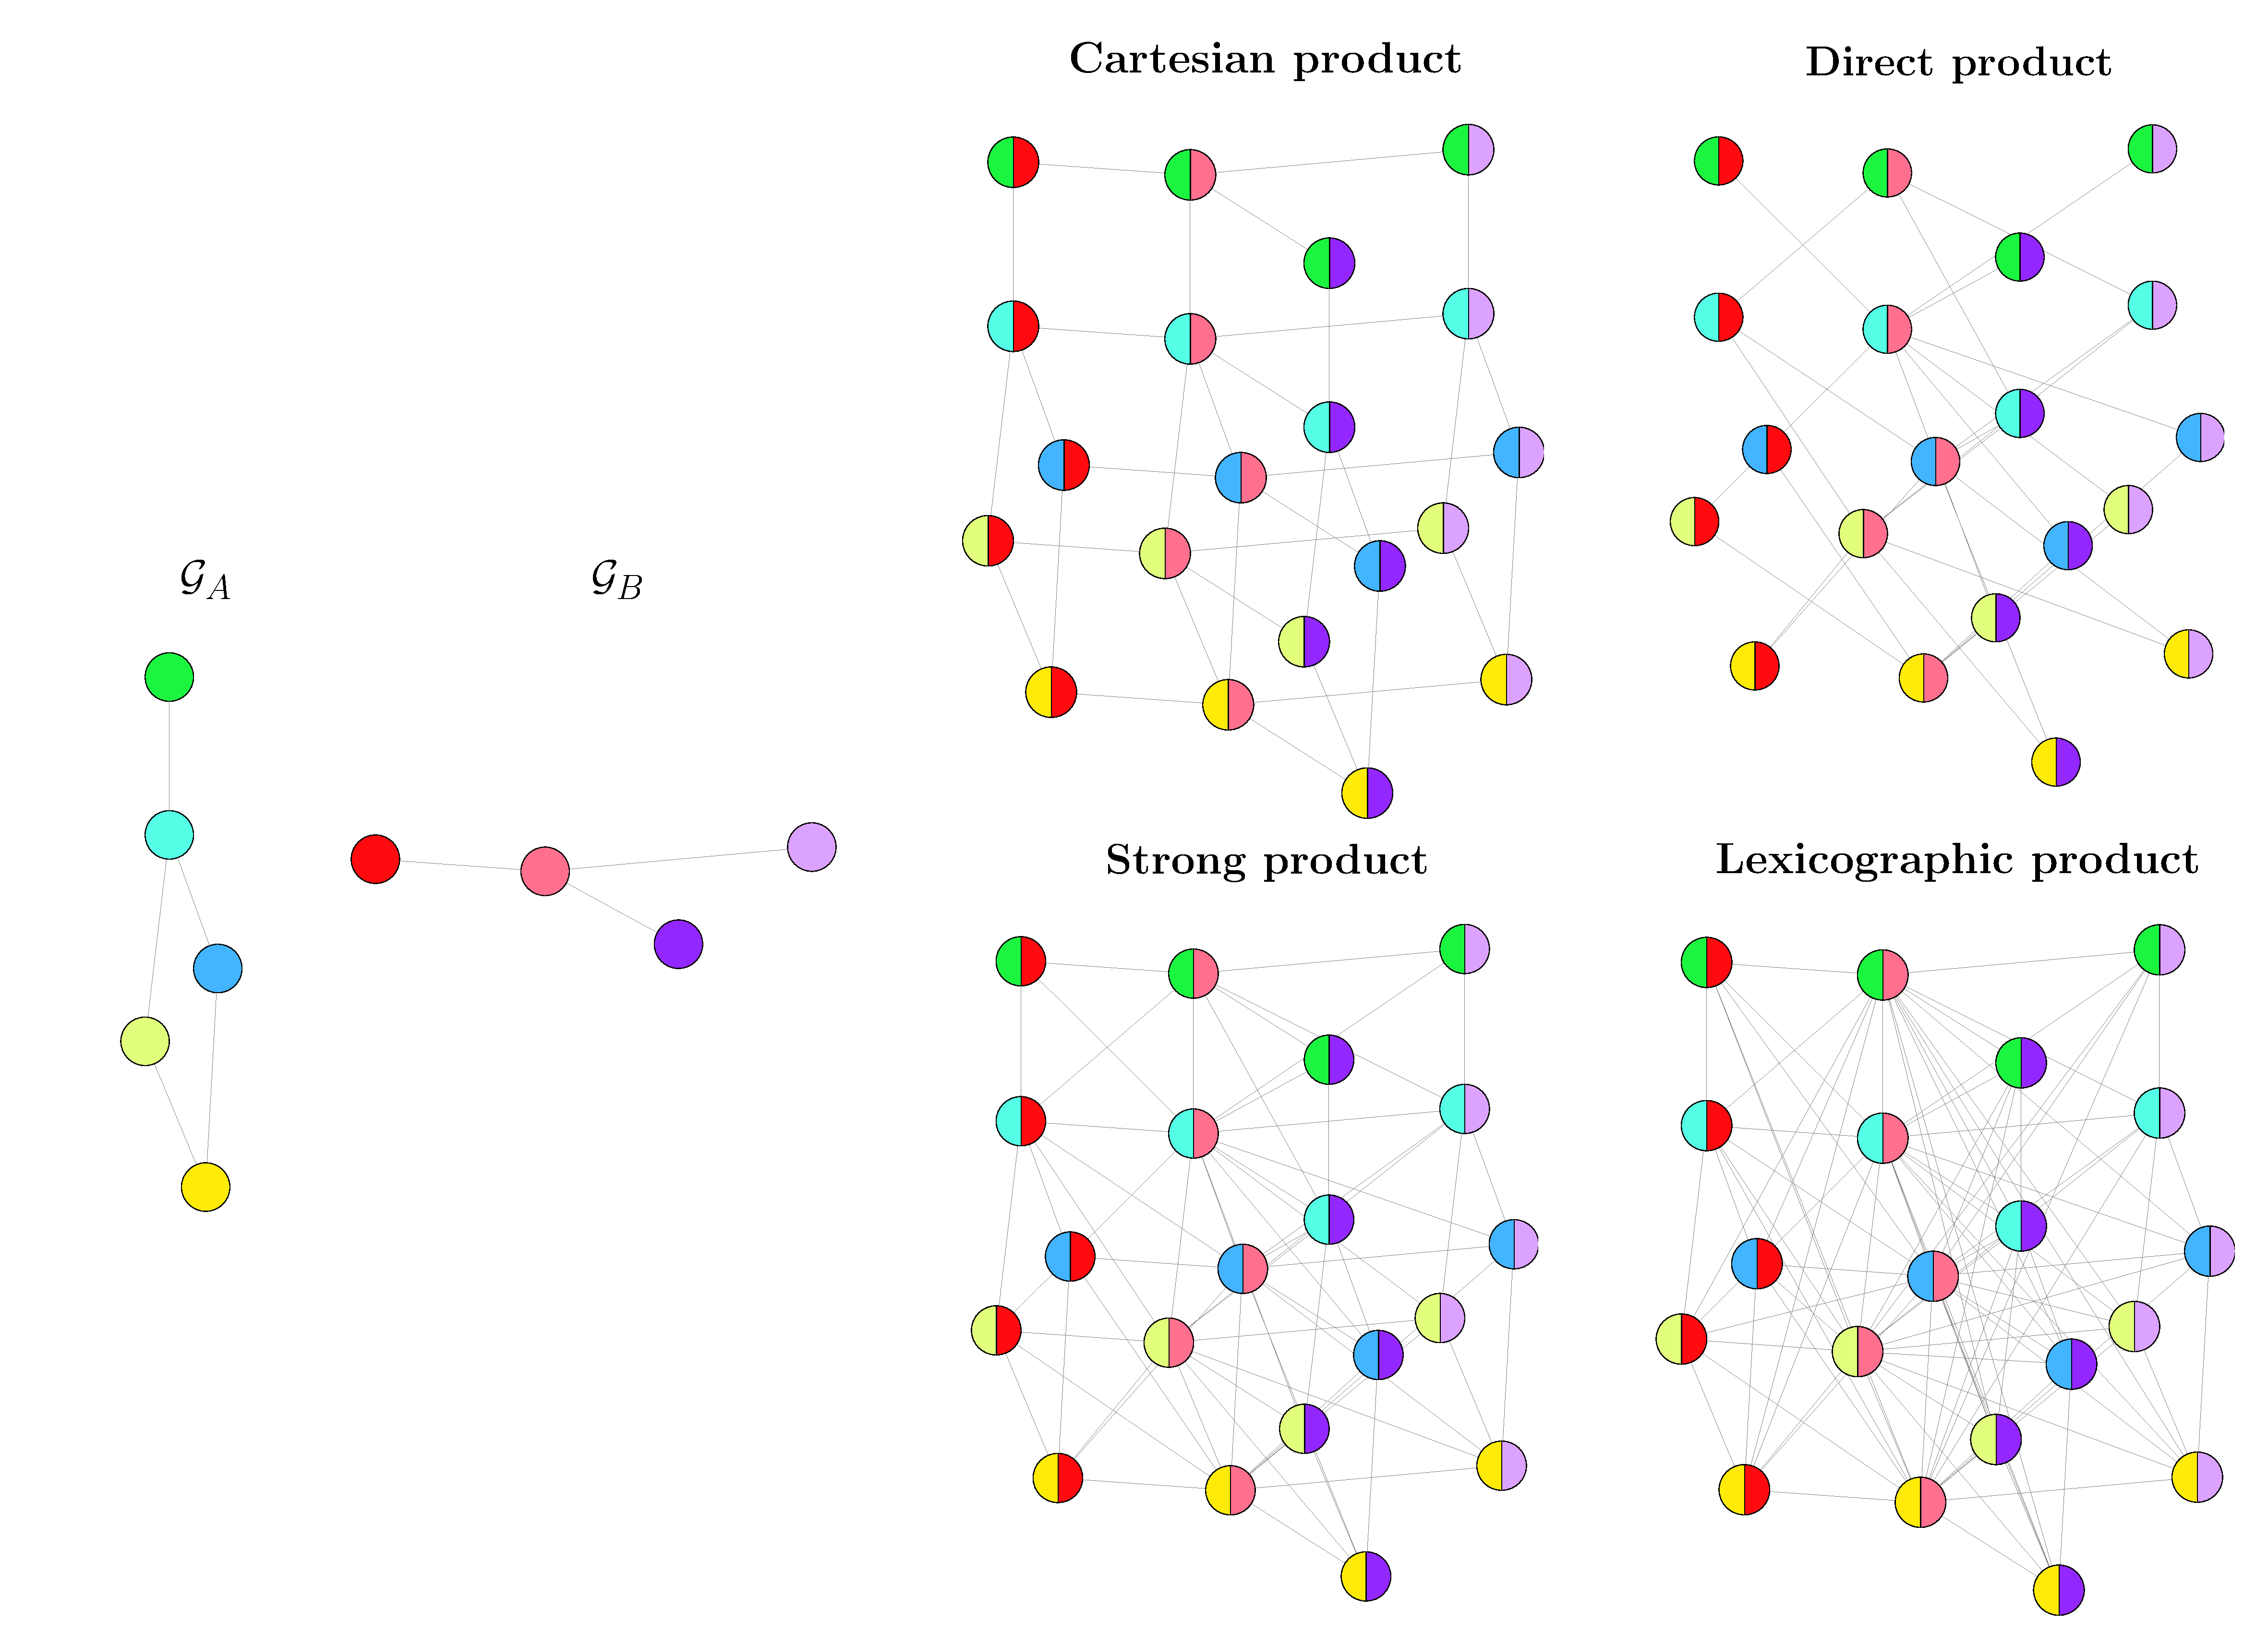
\includegraphics[width=\linewidth]{Figures/product_graphs.pdf}
    \end{center}
    \caption[Graphical depiction of the standard graph products]{A graphical depiction of the four standard graph products}
    \label{fig:graph_products}
\end{figure}


Given these definitions, it may seem that all the standard graph products are non-commutative in the sense that $\A_A \oplus \A_B  \neq \A_B \oplus \A_A $ etc. However, the graphs $\mathcal{G}_A \, \diamond \, \mathcal{G}_B$ and $\mathcal{G}_B \, \diamond \, \mathcal{G}_A$ are in fact isomorphically identical in the case of the Cartesian, direct and strong products. This is not the case for the Lexicographic product \citep{Imrich2000}. 

\subsection{The spectral properties of graph products}

In the field of graph signal processing, we are often concerned with analysing the properties of graphs via eigendecomposition of the graph Laplacian \citep{Mieghem2010}. In the case of product graphs, it is greatly preferable if we are able to fully describe the spectrum of $\mathcal{G}_A \diamond \mathcal{G}_B$ in terms of the spectra of $\mathcal{G}_A$ and $\mathcal{G}_B$ alone. This is because direct decomposition of a dense $\LL$ has time-complexity $O(A^3B^3)$, whereas decomposition of the factor Laplacians individually has complexity $O(A^3 + B^3)$. As the graphs under considerations become medium to large, this fact quickly makes direct decomposition of the product graph Laplacian intractable. However, in the general case, only the spectra of the Cartesian and lexicographic graph products can be described in this way \citep{Barik2018}. In the case of the direct and strong product, it is possible to estimate the spectra without performing the full decomposition (see \citep{Sayama2016}). However, in general, the full eigendecomposition of the product graph Laplacian can only be described in terms of the factor eigendecompositions when both factor graphs are regular. 


Consider the eigendecompositions of $\LL_A$ and $\LL_B$. 

\begin{equation}
    \LL_A = \U_A \LAM_A \U_A^\top, \aand \LL_B = \U_B \LAM_B \U_B^\top
\end{equation}

where $\U_A$ and $\U_B$ are the respective orthonormal eigenvector matrices, and $\LAM_A$ and $\LAM_B$ are the diagonal eigenvalue matrices given by 

\begin{equation}
    \LAM_A = \begin{bmatrix}
        \lambda_1^{(A)}, & & & \\
        & \lambda_2^{(A)} & & \\
        & & \ddots & \\
        & & & \lambda_A^{(A)} \\
    \end{bmatrix}  
    \aand 
    \LAM_B = \begin{bmatrix}
        \lambda_1^{(B)}, & & & \\
        & \lambda_2^{(B)} & & \\
        & & \ddots & \\
        & & & \lambda_B^{(B)} \\
    \end{bmatrix}  
\end{equation}

Given these definitions, table \ref{tab:product_graph_spectra} gives information about the spectral decomposition of the standard graph products.


\begin{table}[h]
    \def\arraystretch{1.8}
    \centering
    \small
    \vspace{0.5cm}
    \begin{tabular}{|l|cc|}
        \hline 
    
        & Eigenvalues
        & Eigenvectors \\
    
        \hline
    
        Cartesian 
        & $\lambda_a^{(A)} + \lambda_b^{(B)}$ 
        & $(\U_A)_a \otimes (\U_B)_b$ \\
    
        Direct$^{\star}$
        & $r_A \lambda_b^{(B)} + r_B \lambda_a^{(A)} - \lambda_a^{(A)} \lambda_b^{(B)}$  
        & $(\U_A)_a \otimes (\U_B)_b$ \\
        
        Strong$^{\star}$
        & $(1+r_A) \lambda_b^{(B)} + (1+r_B) \lambda_a ^{(A)}- \lambda_a^{(A)} \lambda_b^{(B)}$
        & $(\U_A)_a \otimes (\U_B)_b$ \\
    
        \multirow{2}{7em}{Lexicographic$^\dagger$}
        & $B \lambda_a^{(A)}$ 
        & $(\U_A)_a \otimes \mathbf{1}_B$ \\

        & $\lambda_b^{(B)} + B \text{deg}(a)$ 
        & $\mathbf{e}_a \otimes (\U_B)_b$  \\
    
        \hline
    
    \end{tabular}
    \vspace{0.2cm}
    \caption[Spectral decomposition of product graphs]{Eigendecomposition of the Laplacian of the standard graph products. Here, $a$ and $b$ are understood to run from 1 to $A$ and 1 to $B$ respectively. $\star$ only for $r_A$ and $r_B$-regular factor graphs. $\dagger$ note that the lower row forms a full spanning set, but the upper row can also be a useful parametrisation for a subspace. } 
    \vspace{0.3cm}
    \label{tab:product_graph_spectra}
    \end{table}
    

\subsection{GSP with Cartesian product graphs} 

While both the direct and strong products do find uses in certain applications (see \citep{Kaveh2011}), they are both less common and more challenging to work with in a graph signal processing context due to their spectral properties described in the previous subsection. In practice, being limited to regular factor graphs means the majority of practical GSP applications are ruled out. The lexicographic product does not share this drawback, however it is also significantly less common than the Cartesian product in real-world applications. For this reason, in the following, we focus primarily on the Cartesian product. 

Given the spectral decomposition of the Cartesian graph product stated in table \ref{tab:product_graph_spectra}, we can write the Laplacian eigendecomposition in matrix form as follows. 

\begin{equation}
    \LL = \U \LAM \U^\top, \where \U = \U_A \otimes \U_B \aand \LAM = \LAM_A \oplus \LAM_B
\end{equation}

This motivates the following definitions for the Graph Fourier Transform (GFT) and its inverse (IGFT). Consider a signal defined over the nodes of a Cartesian product graph expressed as a matrix $\Y \in \R^{B \times A}$. We can perform the GFT as follows. 

\begin{equation}
    \text{GFT}(\Y) = \MAT{\big( \U_A^\top \otimes \U_B^\top \big) \, \vecc{\Y}} = \U_B^\top \F \U_A
\end{equation}

Correspondingly, we can define the IGFT acting on a matrix of spectral components $\Z \in \R^{B \times A}$ as follows. 

\begin{equation}
    \text{IGFT}(\Z) = \MAT{\big( \U_A \otimes \U_B \big)\,\vecc{\Y}} = \U_B \Z \U_A^\top
\end{equation}


\note{Product graph signals: repseprentation and vectorisation}{

    It is natural to assume that signals defined on the nodes of a Cartesian product graph $\mathcal{G}_A \, \square \; \mathcal{G}_B$ can be represented by matrices (order two tensors) of shape $(A \times B)$. Since product graph operators, such as the Laplacian $\LL_A \oplus \LL_B$, act on vectors of length $AB$, we must define a consistent function to map matrix graph signals $\in \R^{A \times B}$ to vector graph signals $\in \R^{AB}$. The standard mathematical operator for this purpose is the $\vecc{\cdot}$ function, along with its reverse operator $\mat{\cdot}$. However, this is somewhat problematic since $\vecc{\cdot}$ is defined to act in \textit{column-major} order, that is 

    $$
    \text{vec} \left( \begin{bmatrix}
        \Y_{(1, 1)} & \Y_{(1, 2)} & \dots & \Y_{(1, B)} \\
        \Y_{(2, 1)} & \Y_{(2, 2)} & \dots  & \Y_{(2, B)} \\
        \vdots & \vdots & \ddots & \vdots \\
        \Y_{(A, 1)} & \Y_{(A, 2)} & \dots  & \Y_{(A, B)} \\
    \end{bmatrix} \right) 
    =
    \begin{bmatrix}
        \Y_{(1, 1)} \\ \Y_{(2, 1)} \\ \vdots \\ \Y_{(A-1, B)} \\ \Y_{(A, B)}
    \end{bmatrix}
    $$

    As is visible, this does not result in a lexicographic ordering of the matrix elements when the graph signal has shape $(A \times B)$. Therefore, to avoid this issue and to be consistent with standard mathematical notation, we will assume that graph signals are represented by matrices  of shape $(B \times A)$ when considering the product between two graphs. This ensures that matrix elements are correctly mapped to vector elements when using the column-major $\vecc{\cdot}$ function. 

}

\section{Graph Signal Reconstruction on Cartesian Product Graphs}

\label{sec:gsr_cpg}

One task that is of particular interest 

\subsection{A stationary iterative method}

Hello

\subsection{A conjugate gradient method}

Hello

\subsection{Convergence properties}

Hello

\subsection{Image processing experiments}

Hello



\section{Kernel Graph Regression with Unrestricted Missing Data Patterns}

\label{sec:kgr_mdp}

Hello

\subsection{Cartesian product graphs and KGR}

Hello

\subsection{Convergence properties}

Hello


\section{Regression with Network Cohesion}

\label{sec:rnc_mdp}

Hello

\subsection{Regression with node-level covariates}

Hello

\subsection{Convergence properties}

Hello


\section{Multi-Dimensional Cartesian Product Graphs}

\label{sec:nd_gsp}

Hello

\subsection{Fast computation with \textit{d}-dimensional Kronecker products}

Hello

\subsection{Signal reconstruction}

Hello

\subsection{Kernel Graph Regression}

Hello

\subsection{Regression with Network Cohesion}


